%%%%%%%%%%%%%%%%%%%%%%%%%%%%%%%%%%%%%%%%%
% Modified from version 2.1 by RSR
%
% Original author:
% Mathias Legrand (legrand.mathias@gmail.com) 
% With extensive modifications by:
% Vel (vel@latextemplates.com)
%
% License:
% CC BY-NC-SA 3.0 (http://creativecommons.org/licenses/by-nc-sa/3.0/)
%
%%%%%%%%%%%%%%%%%%%%%%%%%%%%%%%%%%%%%%%%%

%----------------------------------------------------------------------------------------
%	PACKAGES AND OTHER DOCUMENT CONFIGURATIONS
%----------------------------------------------------------------------------------------

\documentclass[fleqn,10pt]{SelfArx} % Document font size and equations flushed left

\usepackage[english]{babel} % Specify a different language here - english by default
\usepackage[utf8]{inputenc}
\usepackage{url}
\usepackage{nameref}


%----------------------------------------------------------------------------------------
%	COLUMNS
%----------------------------------------------------------------------------------------

\setlength{\columnsep}{0.55cm} % Distance between the two columns of text
\setlength{\fboxrule}{0.75pt} % Width of the border around the abstract

%----------------------------------------------------------------------------------------
%	COLORS
%----------------------------------------------------------------------------------------

\definecolor{color1}{RGB}{0,0,90} % Color of the article title and sections
\definecolor{color2}{RGB}{0,20,20} % Color of the boxes behind the abstract and headings

%----------------------------------------------------------------------------------------
%	HYPERLINKS
%----------------------------------------------------------------------------------------

\usepackage{hyperref} % Required for hyperlinks
\hypersetup{hidelinks,colorlinks,breaklinks=true,urlcolor=color2,citecolor=color1,linkcolor=color1,bookmarksopen=false,pdftitle={Title},pdfauthor={Author}}

%----------------------------------------------------------------------------------------
%	ARTICLE INFORMATION
%----------------------------------------------------------------------------------------

\JournalInfo{Applied Data Science, 2017} % Journal information
\Archive{Project Report} % Additional notes (e.g. copyright, DOI, review/research article)

\PaperTitle{Smart Homes 1} % Article title

\Authors{Weihua Luo\textsuperscript{1}*, Rabab Alkhalifa\textsuperscript{2}*, Jiayun Wang\textsuperscript{3}*, Nyasha Masamba\textsuperscript{4}*, Boyang Zhao
\textsuperscript{5}* \\
\hspace{2mm} \textit{wl16595} \hspace{14mm} \textit{ra16121} \hspace{15mm} \textit{jw16097} \hspace{12mm} \textit{nm16667} \hspace{19mm} \textit{bz16563} \\
\hspace{4mm} \textit{33891} \hspace{17mm} \textit{31140} \hspace{19mm} \textit{32985} \hspace{17mm} \textit{32928} \hspace{25mm} \textit{33498}} % Authors

%\affiliation{\textsuperscript{1}\textit{Username: wl16595, \quad Candidate number: 33891}} % Author affiliation
%\affiliation{\textsuperscript{2}\textit{Username: ra16121, Candidate number: 31140}} % Author affiliation
%\affiliation{\textsuperscript{3}\textit{Username: jw16097, Candidate number: 32985}} % Author affiliation
%\affiliation{\textsuperscript{4}\textit{Username: nm16667, Candidate number: 32928}} % Author affiliation
%\affiliation{\textsuperscript{5}\textit{Username: bz16563, Candidate number: 33498}} % Author affiliation
\affiliation{*\textbf{Department of Computer Science, University of Bristol.}} 
\affiliation{*\textbf{Repository at \url{https://github.com/smartHomeDataScience}}}

\Keywords{data science, sensor, video, data, programming, visualisation, statistics, machine learning} % Keywords - if you don't want any simply remove all the text between the curly brackets
\newcommand{\keywordname}{Keywords} % Defines the keywords heading name

%----------------------------------------------------------------------------------------
%	ABSTRACT
%----------------------------------------------------------------------------------------

\Abstract{
Sensors, in their many forms, have the ability to transform how people live. Introducing sensors into a home could potentially give us the ability to analyse and subsequently predict frequent activities in order to make homes smarter. In this project, we seek to gain an understanding of sensor data obtained from within a home environment. Using data from a wrist-worn accelerometer, video and depth (RGB-D) data and passive environmental sensors in a home context, we aim to gain insights into the actions and activities conducted by the participants. The data is mainly explored from a visualisation standpoint, and the main deliverable of the project is a web application which enables quick, and easy interactive visualisation of the data.
~}

%----------------------------------------------------------------------------------------

\begin{document}

\flushbottom % Makes all text pages the same height

\maketitle % Print the title and abstract box

\thispagestyle{empty} % Removes page numbering from the first page

%----------------------------------------------------------------------------------------
%	ARTICLE CONTENTS
%----------------------------------------------------------------------------------------

\section*{Introduction} % The \section*{} command stops section numbering
\addcontentsline{toc}{section}{Introduction} % Adds this section to the table of contents
 
This section introduces the problem to be solved, along with associated aims and objectives of the project.
 
	\subsection{The Problem}
This work will use the SPHERE dataset as the basis for analysis. It has been argued that traditional regimes of healthcare are in need of an overhaul to better the experience of patients, relatives, carers and healthcare professionals. Ambient assisted living (AAL) has been proposed as a potential solution. To this end, the EPSRC-funded “Sensor Platform for HEalthcare in Residential Environment (SPHERE)” Interdisciplinary Research Collaboration (IRC) \cite{sphere2015} designed a multimodal system driven by data analytics requirements. The system was tested in one smart homes, and will be deployed in a general population of 100 homes in Bristol (UK). The data from the smart home were collected from the following three primary sensor modalities:
\begin{itemize}
\item Wrist-worn accelerometer and Received Signal Strength Indication (RSSI) data
\item RGB-D cameras (i.e. video with depth information)
\item Passive environmental sensors
\end{itemize}
Accompanying these data are annotations on participant location within the smart home, as well as annotations relating to the activities they were performing at the time. The floor plan of the smart environment is shown in Figure \ref{fig:floorplan}. Nine rooms can be seen in this figure, namely bathroom, bedroom 1, bedroom 2, hallway, kitchen, living room, stairs, study and toilet. In addition, twenty activities of daily living (ADL) are annotated within this dataset. These ADLs are: ascent stairs, descent stairs, jump, walk with load, walk, bending, kneeling, lying, sitting, squatting, standing, stand-to-bend, kneel-to-stand, lie-to-sit, sit-to-lie, sit-to-stand, stand-to-kneel, stand-to-sit, bend-to-stand and turn. The ADLs are further categorised into 1) ambulation activities (i.e., an activity requiring continuous movement, e.g. walking); 2) static postures (i.e., times when the participants are stationary, e.g. standing or sitting); and 3) posture-to-posture transitions (e.g. stand-to-sit, stand-to-bend) \cite{sphere2017}.  \\

\begin{figure*}[!h] \centering
	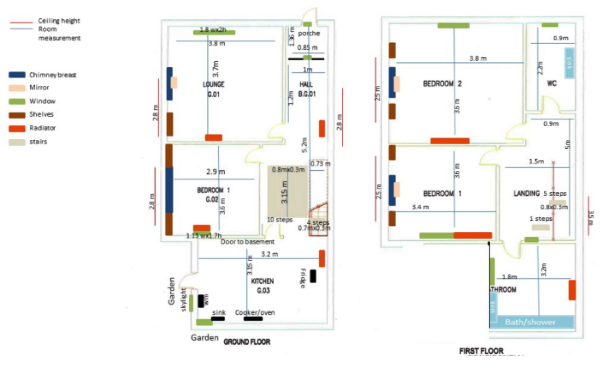
\includegraphics[scale=0.6]{floorplan} 
	\caption{Smart home floor plan \cite{sphere2016}}
	\label{fig:floorplan}
\end{figure*}

Participants in the smart home experiment were asked to follow a script as they performed a variety of tasks around the house. Each participant created a full sequence of sensor data based on the tasks they performed \cite{sphere2016}. The data were received by us as CSV and JSON files. There were testing and training sequences available, but we concentrated on the 10 training sequences as they were complete. Although the data were collected from the same home, they were largely disjointed and could not be easily understood. Hence, the biggest challenge we faced during this project was how we could extract useful information from the seemingly disjointed sensor data, and what added value this useful information would bring.  \\

	\subsection{Aims and Objectives}
The aim of our project is to visually gain insights about participant activities, using sensor data, in order to subsequently aid machine learning predictions. We realised that with these sensor data, we could infer patterns of behaviour. The information derived from these patterns would be helpful for machine learning practitioners (MLP) when making predictions based on the data. For example, they can cross-check new data with the visualisations to find inconsistencies in the new data; or they can visualise the most probable outcomes before training their models, and hence have an inclination to notice when the their models are wrong/making incorrect predictions. The predictions from machine learning could be used to conduct medical diagnoses remotely, energy could be saved when the home is predicted to be vacant, and the home’s layout could be adapted to avoid probable trips and falls. We focused on providing various ways to visualise the data so that an MLP has several tools at their disposal to visualise the data before training a model and making predictions. Our main research questions were:
\begin{enumerate}
\item Can the data be visualised in a quick, easy and interactive way?
\item Are there any unsuspected relationships or inconsistencies in the data that a MLP might find interesting?
\item Can visualisations help MLPs gain higher confidence in their models?
\end{enumerate}
These research questions are congruent with the aim of the project. In order to achieve the aim and answer the questions, we started off with three major objectives. First, we would use diverse preprocessing methods to clean the data in order to make it convenient for us to understand the data. Second, we would employ advanced computational methods to store and retrieve the data. Third, we would use interactive visualisation techniques to dynamically visualise the data, which is the main objective towards solving the problem. \\

	\subsection{Assumptions and Scope}
It was assumed from the onset of the project that we would not be analysing streamed data (from the modalities) in real time. This simplifies the problem and allows us to concentrate on solving the scientific aspect of the problem rather than the infrastructural one. Furthermore, although the solution would be aiming to help MLPs with their work, carrying out the machine learning task is beyond the scope of this project. \\

%------------------------------------------------

\section{Data Science}
This section explains our understanding of the data science field and how data science experiments should be carried out. It gives a glimpse of how we approached the problem of analysing the data.

	\subsection{What is Data Science?}
Data Science is the use of statistics, data analysis and related methods to understand or extract information from data. Other overlapping fields include machine learning and data mining. The most common goal of data science is to extract knowledge from data, or process the data into an understandable structure in order to reach informative conclusions. The data science process usually involves stages such as data collection and storage, data pre-processing, data exploration, data modelling and publishing. \\

	\subsection{Data Science Tools}
As data science has evolved as a discipline, several tools have evolved to serve the needs of data scientists. From proprietary suites such as MATLAB, SPSS and SAS to open source languages such as R and Python, the choices are vast, making it crucial to pick the correct tools for a given project. For our exploratory data analysis, the main tools used were mongoDB (for storage) and Python (for data manipulation). The motivation for selecting these tools is discussed below. \\

\subsubsection{MongoDB}
After data has been collected, it needs to be stored in a form that makes it suitable for future  querying and analysis. CSV files are not very suitable for this; they do not provide a mechanism for external querying of the data. A database was need for this purpose, and mongoDB was chosen as the most suitable datastore \cite{mongo2014}. First of all, the data did not exhibit any complex relationships, so a relational database was not necessary. Furthermore, the ‘schemeless’ nature of mongoDB meant that we did not need to design a schema, freeing up more time for developing the tools to analyse data. Since there was no need for guaranteed consistency, ACID transactions (as featured in relational databases) were also not required. Trading off guaranteed consistency for eventual consistency means that mongoDB is faster than a traditional Structured Query Language (SQL) based database like mySQL. In addition, mongoDB’s indexing capabilities, coupled with its simple query language, made it a great choice when working with several files of time series data. It also handles CSV and JSON file data easily, it is open source, and the data were not being analysed in real time hence there was no need for a real-time datastore. Another option considered for the datastore was CouchDB, but mongoDB seemed more popular and had a larger support community in its favour.  \\

\subsubsection{Python}
An essential part of data science is the need to ‘hack’ and manipulate data. For that, a programming language was needed. We chose Python. The statistical language, R, was also considered. However, Python gave us more scope to achieve our exploratory visualisations where R showed some limitations.  Python has emerged over the last decade as a first-class tool for scientific computing tasks, including the analysis and visualisation of large datasets. In particular, the usefulness of Python for data science stems primarily from the large and active ecosystem of third-party packages, a number of which were used in this project: Pandas dataframe for manipulation of data ingested from mongoDB, Matplotlib for publication-quality visualisations, Bokeh for interactive web app visualisations (similar to D3.js) and ffmpeg for video data synthesis. Many other tools used during the project, such as Jupyter notebooks, also work with Python and provide the computational environment in which many data scientists work \cite{Vanderplas17}. \\

\section{Data Science System Architecture}
This section elaborates on how the deliverables were created through each stage in the data science process.

	\subsection{Storing and loading data}
After choosing mongoDB as the database to store the data (as the smart home data is in CSV and JSON format), the advantages of mongoDB started to become apparent as the datastore had a highly flexible storage format. This meant we could handle and store both CSV and JSON data conveniently during the data storage process. The other advantage of mongoDB, i.e. that it performs at a relatively high data I/O operation speed also came in handy. As we were planning to construct an interactive visualisation tool, the speed of data reading from the database and the strength to ensure the stability of  the data’s structure  were crucial for the performance of visualisation tool. Figure \ref{fig:sys-arc} shows the planned structure of how stored data was going to be loaded into the web app for interactive visualisation. \\

\begin{figure}[!h] \centering
	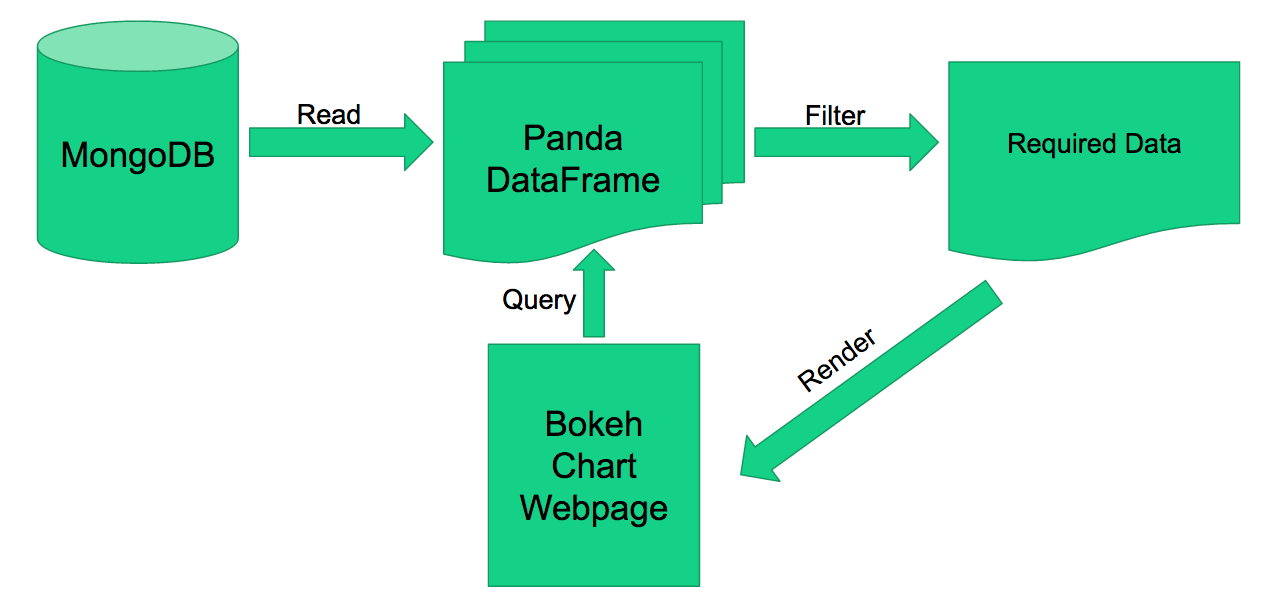
\includegraphics[scale=0.2]{sys-arc} 
	\caption{System architecture}
	\label{fig:sys-arc}
\end{figure}

Data will be ingested from the mongoDB datastore and manipulated using the Pandas dataframe. An incoming query from the web app will produce filtered data from the dataframe, which will subsequently be rendered by the Bokeh library on the web page. \\

	\subsection{Data wrangling}
\subsubsection{Data cleaning}
Because the data received from the SPHERE project had already been largely cleaned, the main reason for performing the data cleaning stage was to remove outliers. Our method was to first plot the data, which makes it easy to visually notice the outliers. To clean the acceleration data, of which the $ x, y, z $ axes represent the coordinates of the accelerometer, we worked from the assumption that the accelerometer (bound to the wrist) moved within a fixed size space. So, our method of finding the outlier was to plot the coordinate of all data in a 3-dimensional space. Figure \ref{fig:outliers} shows the result of the acceleration data. The outliers can be recognized distinctly from the figure. Different colours indicate different rooms. \\

\begin{figure}[!h] \centering
	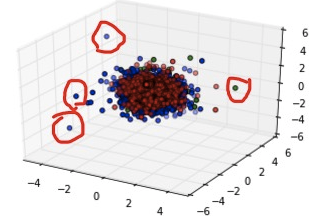
\includegraphics[scale=0.5]{outliers} 
	\caption{Outlier detection}
	\label{fig:outliers}
\end{figure}

Further work to find the outliers existing in the RSSI signal within the acceleration data file is based on aggregation of the file with location data, which will be discussed in more detail below. The idea is that the sensor reflecting strongest signal should be the nearest one to the participant. Hence, if we check the signal strength with respect to location, the outlier data will be uncovered by showing the expected and actual sensor presenting strongest signal strength. \\

\subsubsection{Missing data}
We focused on the acceleration data for missing data management, where the signal reading of sensors in some rooms was missing from the data. After intensive observation of the data, we found that the missing data points were likely due to the fact that there was no signal received from the sensor in question. This  means there was somehow a loss of signal data (possibly due to hardware failure, or maybe the participant was completely out of the sensor’s range). However, the problem was that these missing data would cause problems in the next steps of our study. By running a statistical count algorithm, we found the missing data of each column to be as shown in Table \ref{table:missing-data}. \\

\begin{table}[h!]
\centering
\begin{tabular}{ |c |c |  }
\hline
Data column & Count of missing data \\
\hline
$ x $ & 0 \\
$ y $ & 0 \\
$ z $ & 0 \\
Kitchen\textunderscore AP & 24,317 \\
Lounge\textunderscore AP & 14,160 \\
Upstairs\textunderscore AP & 20,985 \\
Study\textunderscore AP & 35,710 \\
\hline
\end{tabular}
\caption{Missing data from acceleration file}
\label{table:missing-data}
\end{table}

With the exception of the $ x, y, z $ coordinates in the acceleration data, there is a huge amount of missing data of the other three data. The Study{\_}AP data is completely empty (we were informed to disregard this by SPHERE project member). In order to solve the missing data problem, we calculated the mean, standard deviation, minimum and maximum values of the data. We also found where the first quartile, median, and third quartile thresholds of the original data were. The data in Figure \ref{fig:md-stats} shows our results. We found that the maximum and minimum were not good enough to fill up the gap, because they are extreme values. However, using the mean of the column as the value to fill the gap had the effect of reducing the error and standard deviation, so we used the column mean to address missing values in the data. \\

\begin{figure*}[!h] \centering
	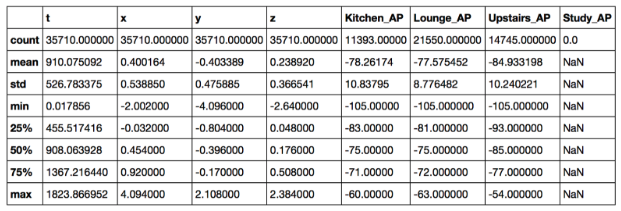
\includegraphics[scale=0.6]{desc-stats} 
	\caption{Descriptive statistics for each data column}
	\label{fig:md-stats}
\end{figure*}

\subsubsection{Data aggregation}
After intently studying these diverse data for a while, we found the key index of all the different data documents is time(t). Hence we focused on integrating the annotation data and location data together in one collection, based on time. For example, the location file has detailed entries of each record while the annotation data has short entries of each record. The common element between them was time. We realised that if we split each record in the two files by time, the time field would make it convenient for us to combine the two data documents. Such aggregation of data was the foundation for us to research the relationship between the two types of data and to prepare the data for visualisation. An illustration of this method is shown in Figure \ref{fig:data-agg}. \\

\begin{figure}[!h] \centering
	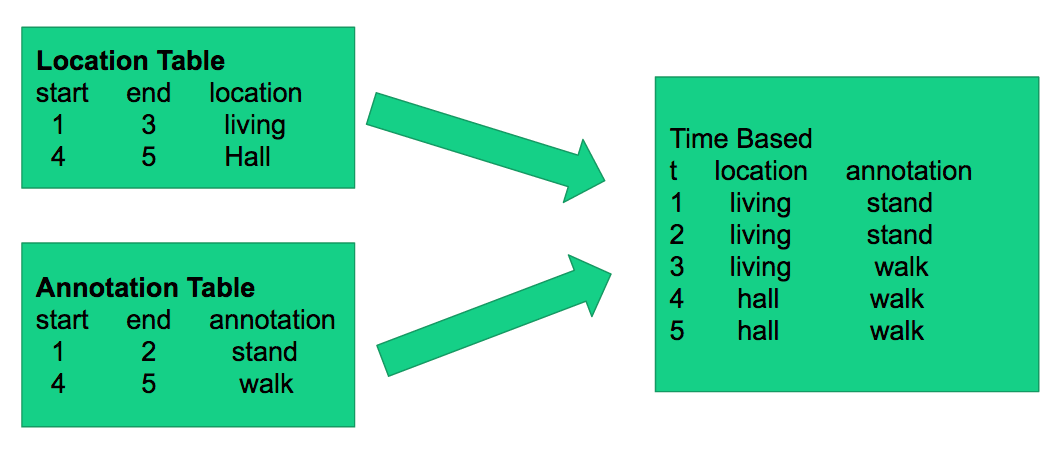
\includegraphics[scale=0.2]{data-agg1} 
	\caption{Data aggregation by combining tables}
	\label{fig:data-agg}
\end{figure}

We also used time as the key index to aggregate other files such as the acceleration data with location data; and also to aggregate the three video files in each complete sequence. The former was in preparation for finding the relationship between the accelerometer signal and location. The latter was in preparation for finding the flow of video data through each sequence, and the aggregation is depicted in Figure \ref{fig:data-agg2}. First, we merged all video files (kitchen, living room, hallway), ensuring they were correctly labelled (by location). We noticed from the data that the difference between each data point in the video files was 0.3 seconds. Hence we adapted the time field in the location{\_}0 file to discrete time intervals which were 0.3 seconds apart. Finally, we sorted the entries (by time). \\

\begin{figure}[!h] \centering
	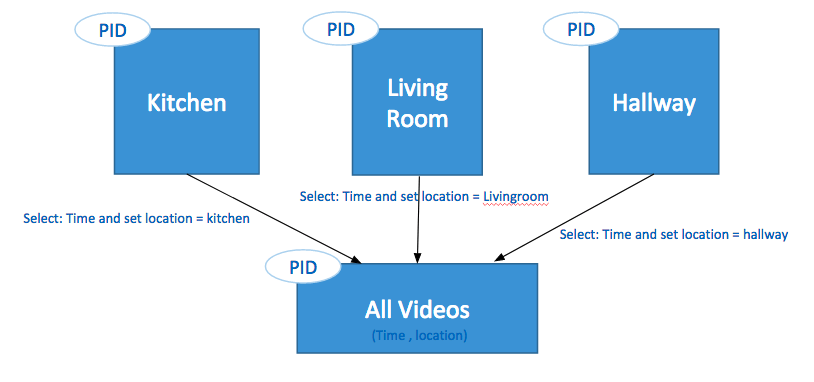
\includegraphics[scale=0.3]{data-agg2} 
	\caption{Data aggregation of video files}
	\label{fig:data-agg2}
\end{figure}

	\subsection{Data exploration and visualisation}
\subsubsection{Web app interactive visualisation}
We produced an exploratory web interactive visualisation application which is able to dynamically present information about participant activities, as shown in Figure \ref{fig:webapp}. The location of a participant can be seen interactively in the floor plan as time progresses (using a time slider). A Gantt chart is created to show the location of the participant, and a MLP using the app is able to choose which person they want to observe. There are also statistical analyses of the location data and annotation data by 2-dimensional and 3-dimensional histograms. When the page loads, the statistics for all 10 training sequences are loaded. From there, the user can also decide the room or the Person ID whose statistics they would like to see. The 3-dimensional histogram shows the pattern between annotation and location, which can be customised by changing the Person ID or choosing all of the participants for example.  Meanwhile, the 2-dimensional histogram shows the statistical data of the annotations/ADLs, also interactively customisable by changing the Person ID and/or location. \\

\begin{figure*}[!h] \centering
	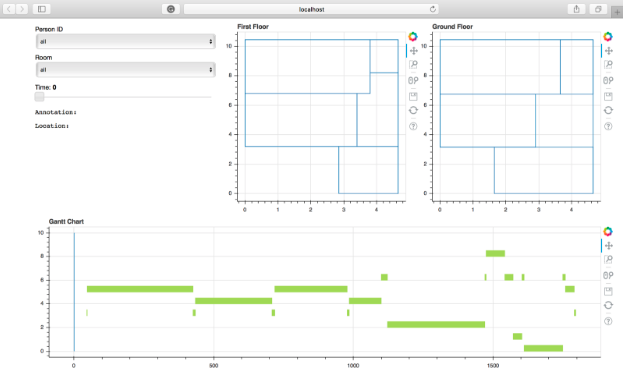
\includegraphics[scale=0.8]{webapp1} 
	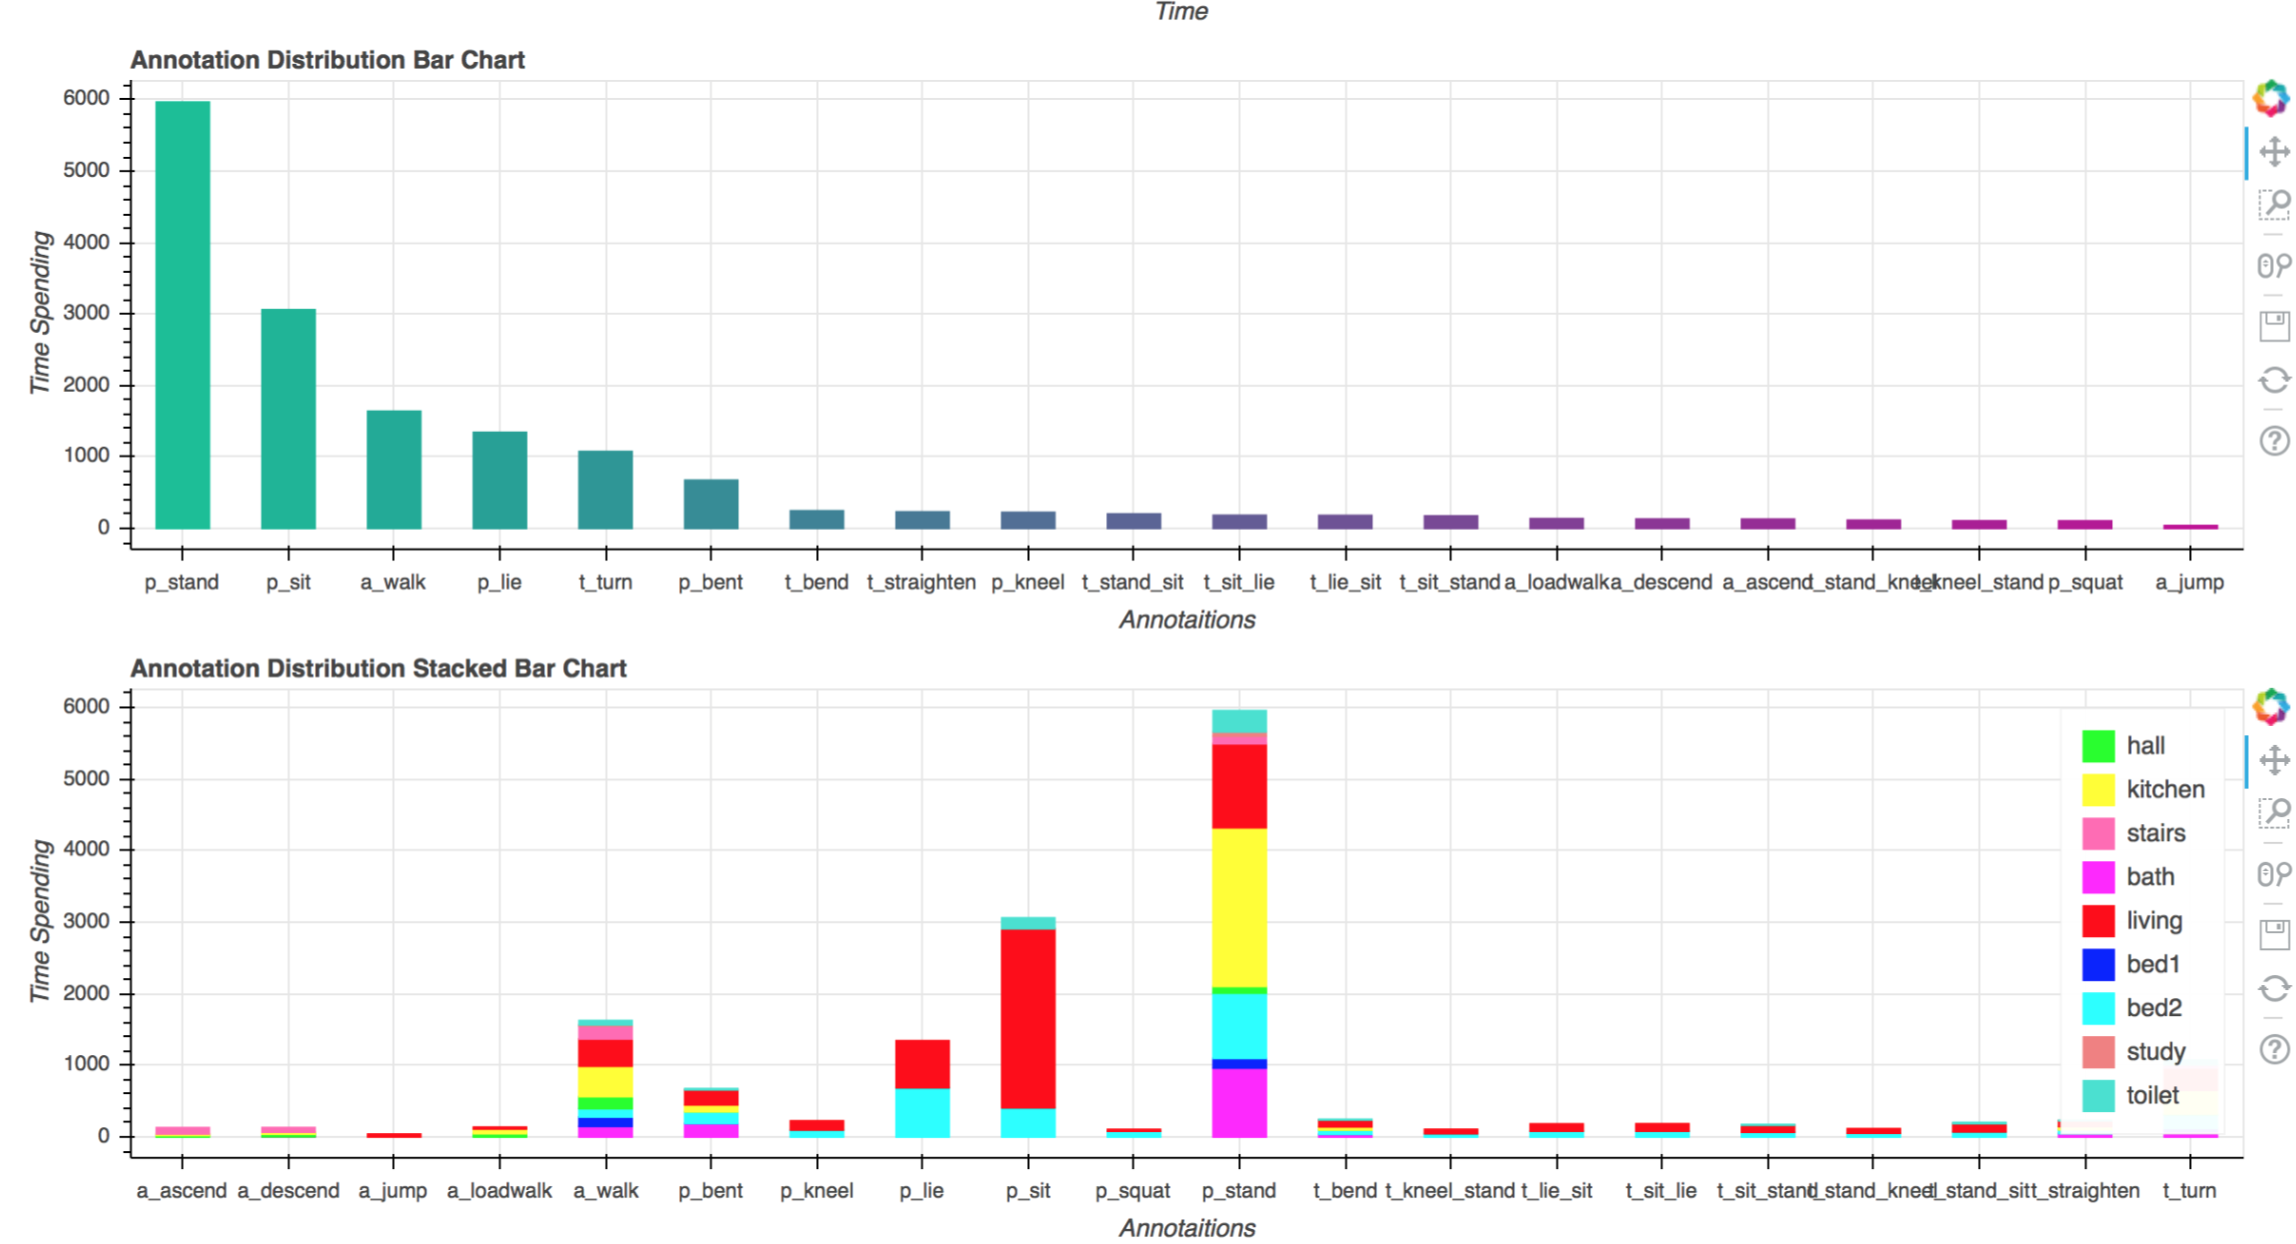
\includegraphics[scale=0.425]{webapp2}
	\caption{Web application interactive visualisation}
	\label{fig:webapp}
\end{figure*}

To aid clarity on some of the functionality, Figure \ref{fig:slider} shows an examplary depiction of the dynamic behaviour of a participant in living room as time is moved (on the time slider). \\

\begin{figure}[!h] \centering
	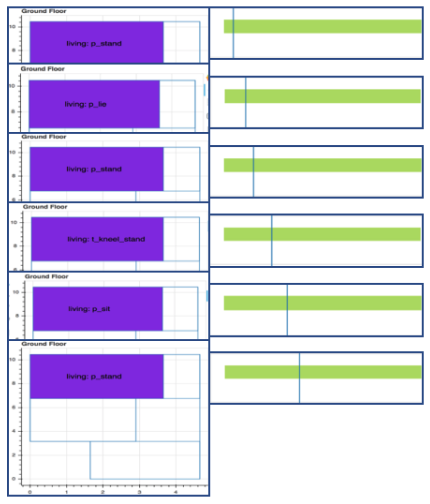
\includegraphics[scale=0.5]{slider} 
	\caption{Illustration of dynamic behaviour with time}
	\label{fig:slider}
\end{figure}

\subsubsection{Video visualisation}
Since video data came in the form of bounding box coordinates (for participants’ privacy), the MLP would benefit from viewing something more friendly to the human eye to see, in a real-life setting, how some parts of a sequence happened. Hence, the video visualisations were a creative way to solve this problem, particularly considering the location photograph in the background dynamically changes as the model of the participant (a red box) also moves around the home. Figure \ref{fig:video} shows what the video visualisation tool looks like. Note that in real life, this visualisation shows dynamic backgrounds and motion of the bounding box as time progresses. \\

\begin{figure}[!h] \centering
	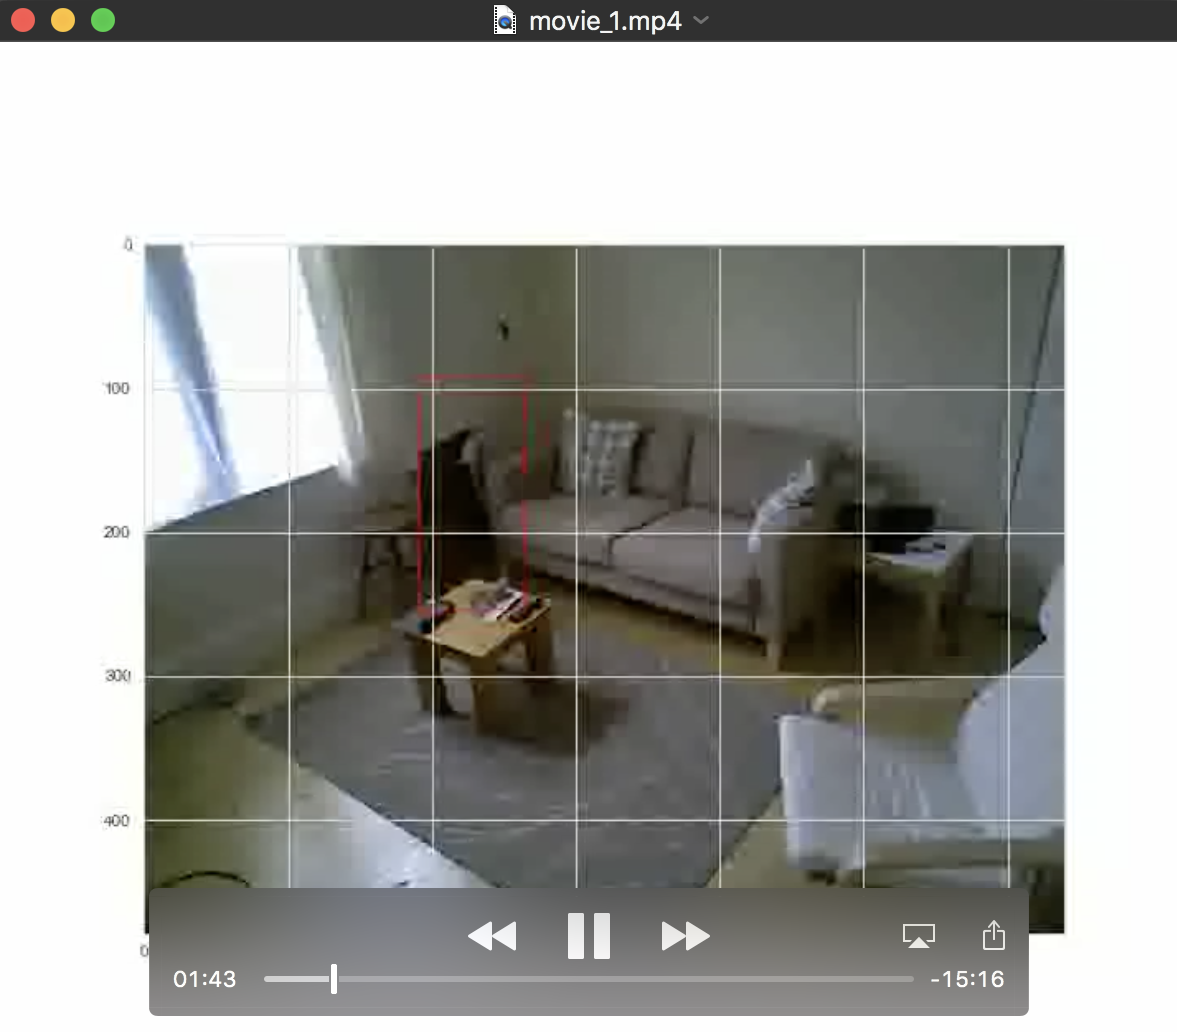
\includegraphics[scale=0.4]{video} 
	\caption{Still image of video visualisation}
	\label{fig:video}
\end{figure}

\subsubsection{Jupyter notebook visualisations}
The Jupyter notebooks allowed interactive execution and sharing of Python code, and supplemented the two forms of visualisation above by allowing interactive graphing of the data. Most of the stand alone figures included above were created in Jupyter notebook. Due to the interactivity of Jupyter notebooks, we could write code that could easily be changed for further visualisation by the MLP as and when needed. For example, to investigate if all sequences are the same, the MLP could plot two gantt charts next to each other, such as in Figure \ref{fig:seq-comp} below. \\

\begin{figure}[!h] \centering
	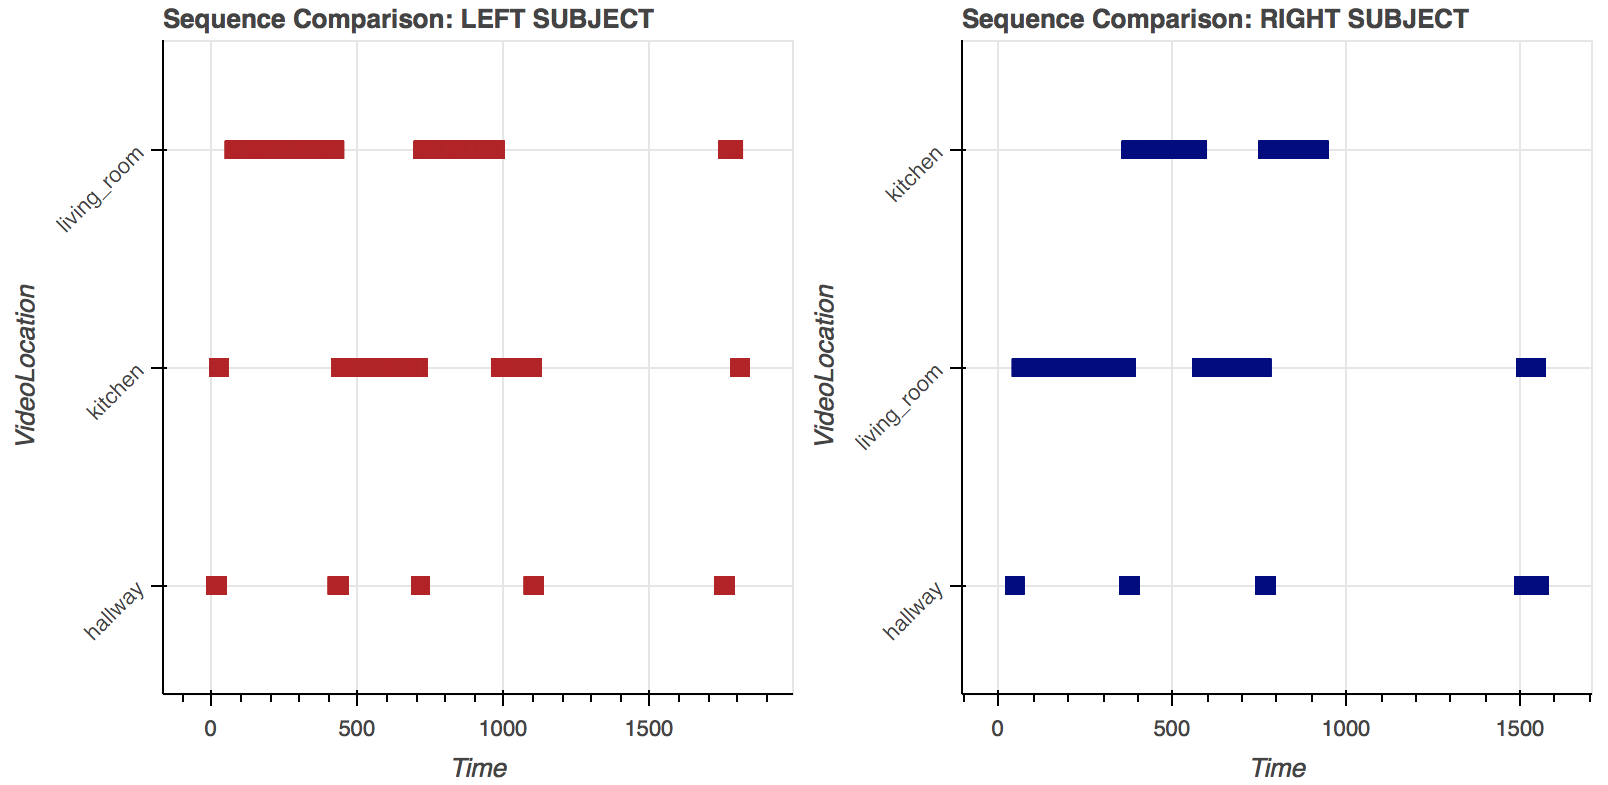
\includegraphics[scale=0.3]{seq-comp} 
	\caption{Sequence comparison in Jupyter notebook}
	\label{fig:seq-comp}
\end{figure}

Plotting RSSI strength data overlaid with the triggered access point (location) also became possible, as can be observed in the notebook visualisation in Figure \ref{fig:rssi-signal}. This enabled us to see relationships between the RSSI values and the triggered access point. 

\begin{figure*}[!h] \centering
	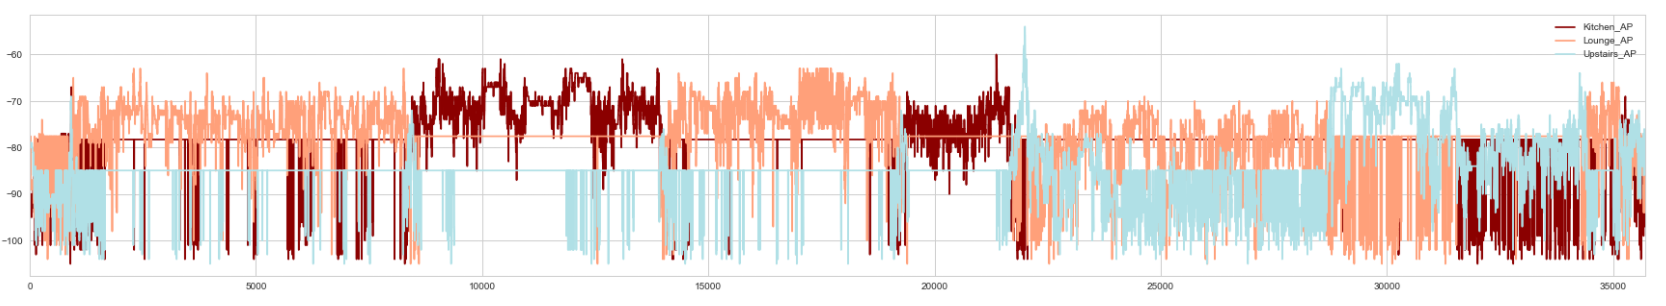
\includegraphics[scale=0.6]{rssi-signal} 
	\caption{RSSI strength vs location}
	\label{fig:rssi-signal}
\end{figure*}


	\section{Results}
This section presents our observations as seen from the data science tools we built.
\subsubsection{Web app}
The web application, which is the MLP’s main tool, allows interactive analysis of each person’s behaviour, or the behaviour of all the training sequences as a whole. Listed below are a few generalisations made from the interactive visualisation:
\begin{enumerate}
\item It is apparent from the dynamic gantt chart that all the participants spend the most time in the living room, followed by the kitchen. They also spend the least amount of time in the toilet, bath room, study room and bedroom 1. Almost all the time, participants walk and stand in these rooms except occasional sitting in the toilet. 
\item Participants are sitting in the living room most of the time. What is interesting is that they do not sit continuously for a long time, but rather they frequently stand up and sit down as time progresses, accompanied by a little walking. Conversely, participants spend more time standing in the kitchen accompanied by occasional walking. Combining with the finding in the video visualisation, participants take a lot of time standing before the cooker/doing some kitchen work.
\item A significant finding is the difference in behaviour of participants in bedroom 1 and 2. Participants never lie and sit in bedroom 1 but spend most time sitting and lying on the bed in bedroom2. This finding is able to distinguish the location of the person.
\item When the participant shows a behaviour of sitting, he only has the possibility to be in living room, bedroom2 or toilet. But participants sit more than lying in the living room and show opposite behaviour in bedroom 2. Meanwhile, they never lie in the toilet. This finding is able to help distinguishing the location in these three rooms.  
\item  A unique behaviour of participants in the living room is jumping. From observing the app visualisation, it is determined that participants never jump in other rooms.
\item The participants spend little time in bedroom 1. All participants only enter the room, walk around and turn around swiftly then leave the room.
\item Participants generally just walk in the hall without turning around (almost all the time). This is in contrast the behaviour exhibited in bedroom 1.
\item The participants only descend or ascend in the stair area. That is  the sole activity in the stair area.
\end{enumerate}

\subsubsection{Video}
Videos give the MLP a way to see exactly how a person moved around the home in a life-like manner. On observing the videos along with the video data, we observed the following:
\begin{enumerate}
\item The camera can only detect the moving part of the body, so the bounding box in the video sometimes can be deceivingly small representing only some partial body detection.
\item Some video data are missing, presumably because the person is in a different room at the time, meaning the bounding box coordinates would have been recorded as zero values and then subsequently removed when the data were cleaned.
\item The camera/bounding box sometimes struggles to capture people’s frames accurately, for example when they are standing in front of a window, only the upper part of their body is detected. Maybe that is because only the head is moving (albeit slightly).
\item The video flow was smooth, suggesting the data capture equipment had a high degree of  accuracy .
\end{enumerate}

\subsubsection{Jupyter notebook}
The Jupyter notebooks give the MLP a way to visualise the data interactively. Some of the observations that can be made using this tool are as follows:
\begin{enumerate}
\item By plotting two video sequences side by side, it can be observed, that the video data for the participant on the left and the participant on the right are different. Hence, the way in which they performed the script is also different. All the MLP has to do to come up with this visualisation is to change two lines of code, which is very handy. 
\item By comparing the merged video data from the three locations against all other location data as measured by the environmental sensors in Jupyter notebook. We observed that because the data are clean, the time sequences are complementary and generally do not intersect. In fact, they show the progression of the time sequence as the person performed the tasks, as seen in Figure \ref{fig:vidnloc} below. The coloured shapes represent video data (blue - living room; green - hall; red - kitchen), and the thicker the shape, the more video data available. As can be seen from the figure, the person (ID 1) travels from the living room through the hall to the kitchem, then back to the living room and so forth until the sequence completes in the hall.  \\
 
\begin{figure}[!h] \centering
	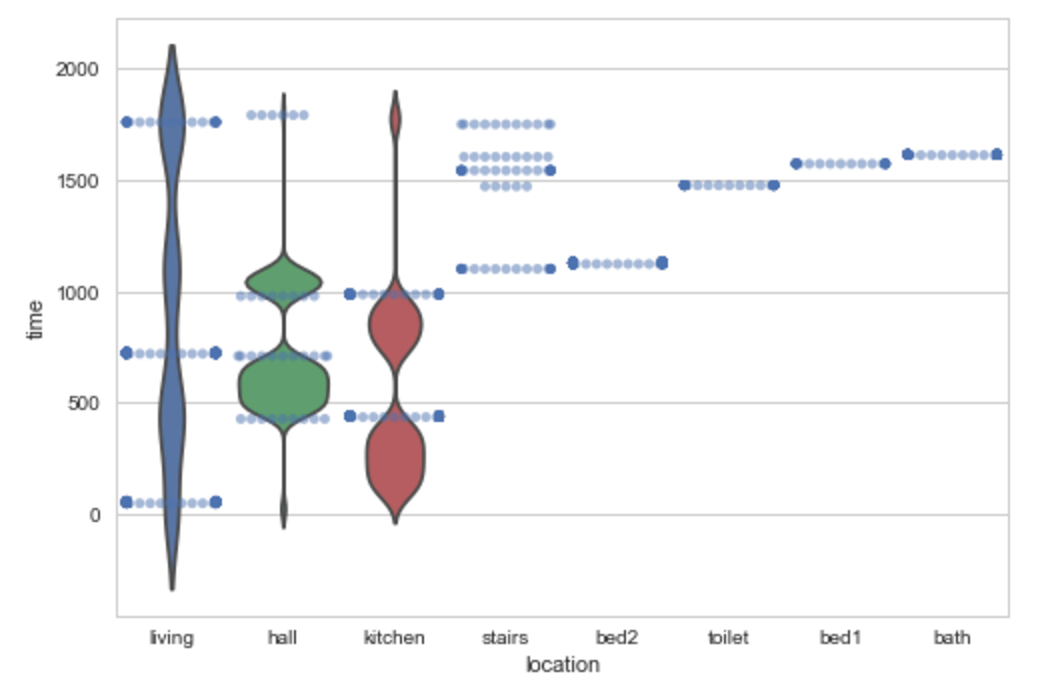
\includegraphics[scale=0.5]{vidnloc} 
	\caption{Video data vs location data}
	\label{fig:vidnloc}
\end{figure}

\end{enumerate}

	\section{Insights}
This section provides an evaluative analysis of the insights and generalisations we made from our observations. 
\begin{itemize}
\item By considering the floorplan and the list of ADLs together, it should be clear to see that there are correlations between these: since there is no seating area in the kitchen, it is very unlikely that somebody will sit in the kitchen. However, since there are many seats in the living room, it is much more likely that somebody will sit in the living room than in the kitchen. Additionally, one can only ascent and descent stairs when one is on the staircase. It is also obvious that the signal strength of sensors in different rooms, to a extent, reflects the location of participant, as the nearest sensor should receive the strongest signal. This potential relation is worthy of deeper scrutiny so as to be able to articulate the relationship in a more precise way.
\item In some instances, the location cannot be precisely determined. PIR sensors can elicit false negative and false positive activations - i.e., they do not always trigger when someone is present, and they can trigger when someone is not present due to the infrared radiation from the sun in warm weather. Video data obtained from across the whole house would have gone a long way to solving this location issue, as the camera does not suffer from the same problems. The MLP can have more confidence about the location of a participant if they are in a location which is fitted with a camera. The association rule might look like the following:

IF (kitchen PIR sensor activated) and (kitchen video activated) THEN Location = Kitchen

Once a location is known, we can consequently have more confidence in the likely activity being done, if we also consider annotations. For example, the association rule in this case would become:

IF (kitchen PIR sensor activated) and (kitchen video activated) THEN ADL = standing

The above could be used by the MLP to infer that the participant could be cooking or washing plates at that particular time, for example. Furthermore, both location and ADL could be targets for machine learning classification.
\item After we aggregated the acceleration data and location data by time, we realised there is a relationship between signal strength and location. Combining with the room map and the sensor location, the patterns we extracted are as follows:

IF(the signal strength in lounge sensor is the strongest) and (the signal strength in other two sensors is weak) THEN the location = living room.

IF(the signal strength in kitchen sensor is the strongest) and (the signal strength in other two sensors is weak) THEN the location = kitchen.

IF(the signal strength in lounge sensor is around 100 ) and (the signal strength is around 70-75) and (the signal strength in kitchen is missing or around 78) THEN the location = bedroom 1

IF(the signal strength in upstair sensors is around 85-100) and (the signal strength in lounge sensors is around 70-90) and (the signal in kitchen is missing) THEN the location = bedroom 2

IF(the signal strength in upstair sensors is around 65-70) and (the signal strength in lounge sensors is around 85-100) and (the signal in kitchen is missing or around 100) THEN the location = toilet

IF(the signal strength in upstair sensors is around 70) and (the signal strength in lounge sensors is around 90-100) and (the signal in kitchen is missing or around 100) THEN the location = stairs

IF(the signal strength in upstair sensors is around 85-100) and (the signal strength in lounge sensors is around 75-100) and (the signal in kitchen is around 70-100) THEN the location = hall
\item From behaviours of all participants, several patterns can be extracted from the observation of the web tool above.

IF(the participant is sitting down and standing up alternatively ) THEN the location = living room

IF(the participant is standing more than 250 seconds) and (the participant is never sit down) THEN the location = kitchen

IF(the participant spend more time in sitting down more than in lying) THEN the location = living room

IF(the participant spend more time in lying more than in sitting down) THEN the location = bedroom 2

IF(the participant only sit down but never lie) THEN the location = toilet

IF(the participant is jumping) THEN the location = living room

IF(the participant spend most time for walking and loadwalk) THEN the location = hall

IF(the participant has behaviours of descend and ascend) THEN the location = stairs

IF(the participant only stands, walks and turns in a continuous manner) THEN the location = bedroom 1
\end{itemize}

\section{Future Work}
Future work will largely be devoted to performing activity and location recognition using machine learning on the data, using the insights gained from this data science process. A number of features make this dataset valuable and interesting to MLPs \cite{sphere2017}: 
\begin{itemize}
\item It features missing data.
\item The data are temporal, and correlations in the data must be captured either in the features or in the modelling framework. 
\item There are many correlations between activities. 
\item The problem can be modelled in a hierarchical classification framework. 
\item The targets (ADLs) are probabilistic (since the annotations of multiple annotators were averaged). 
\item The optimal solution will need to consider sensor fusion techniques.
\end{itemize}
Given more time, it would have been interesting to tackle the problem further and build a tool for the MLP that analyses the raw sensor data and predicts the activity, based on parameters set by the MLP. For example, the tool could have looked something like the MATLAB suite shown in Figure \ref{fig:full_screen} \cite{Mathworks2015}. It takes in accelerometer data as an input, trains a neural network, predicts/estimates the ADL, calculates statistical correlations between activities, and even produces a pre-trained model in C++ for use outside the MATLAB environment. Such tools would greatly complement the tools we have already provided to the MLP. \\

\begin{figure*}[!h] \centering
	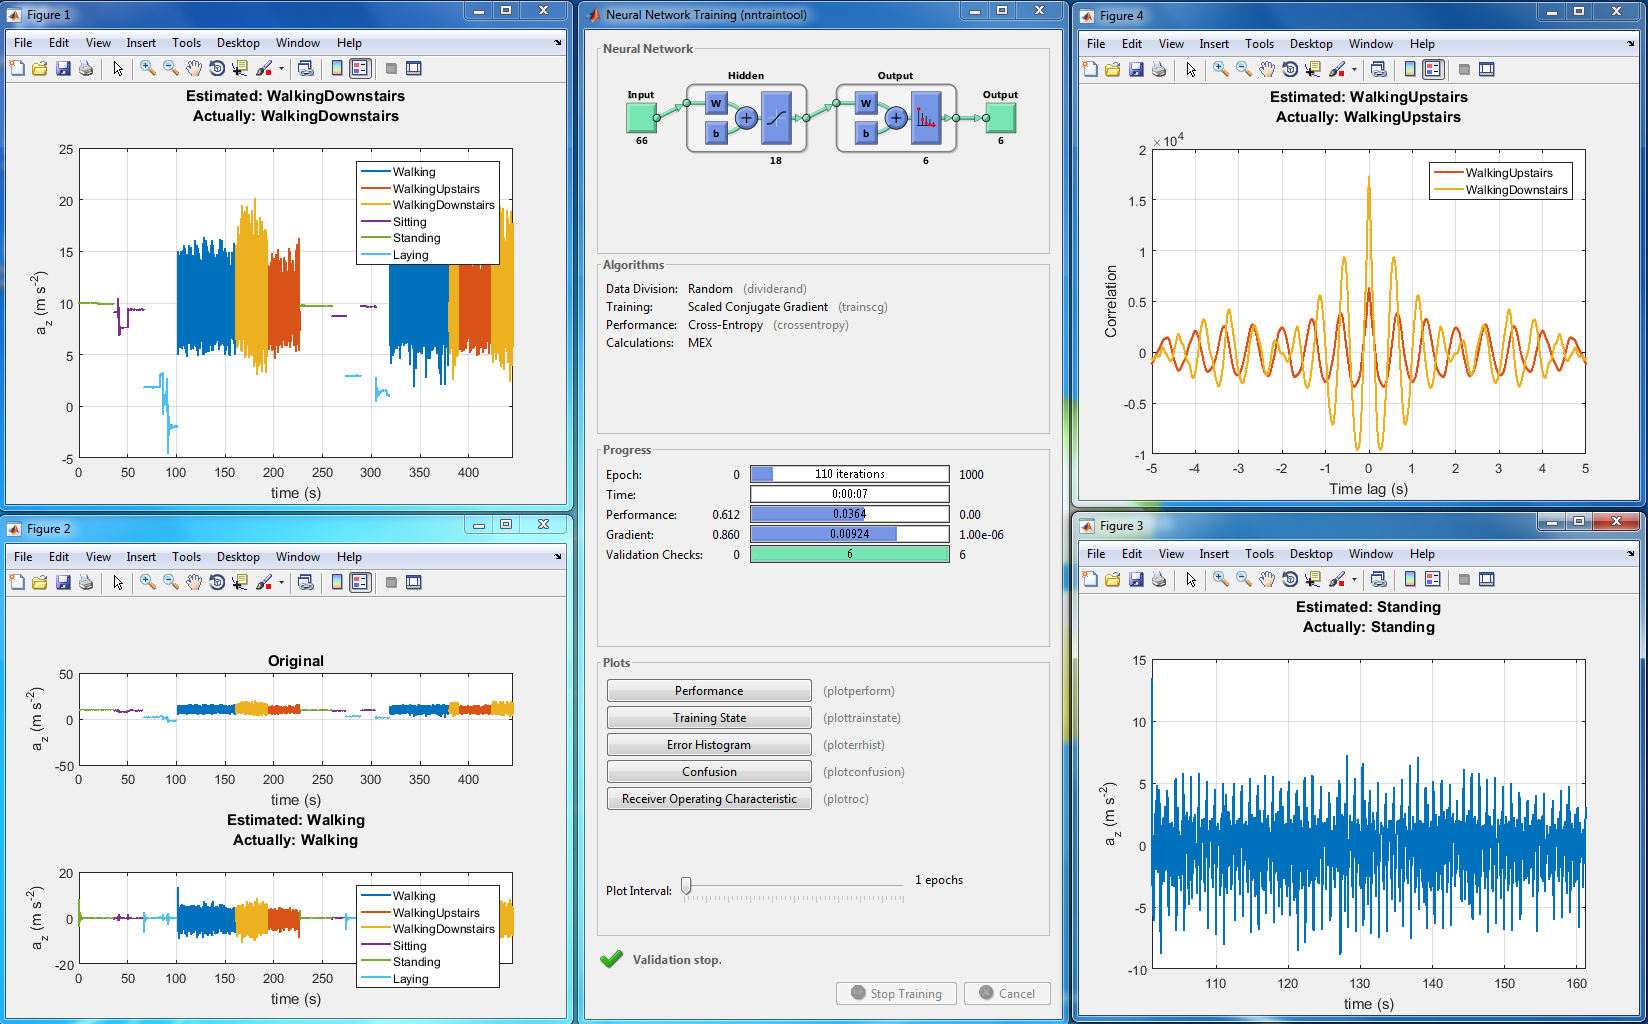
\includegraphics[scale=0.4]{full_screen} 
	\caption{MATLAB neural network activity recognition suite \cite{Mathworks2015}}
	\label{fig:full_screen}
\end{figure*}

\section{Conclusion}
Like any well-thought out data science experiment, we started off with three central questions in order to guide our aims and objectives. In this section, we will study of these questions to determine if the aim of the project has been achieved. \\

The first question pondered whether the sensor data we had been given could be visualised in a quick, easy and interactive way. The answer to this question is a resounding yes. In this project, we have delivered a suite of three tools which can visualise different aspects of the data to aid a machine learning researcher make sense of the data before using the machine learning data for their machine learning predictions.\\

The second question wondered if there were any unsuspected relationships or inconsistencies in the data that a MLP might find interesting. Using the tools we built, we found quite a few of these. Each tool we derived found some interesting patterns. For example, the web app visualisation enabled us to find out that jumping only takes place in the living room, therefore the MLP can say with a high probability that if jumping is detected by the sensors, the participant is likely to be in the living room. The video found that the bounding box is unreliable when the participant is standing next to a window; however the flow is typically smooth so the video equipment generally exhibits a high degree of accuracy. The Jupyter notebooks enabled us to see when sequences were different, enabling the MLP to compare these sequences and get a general sense of how scripts were performed differently by the participants without even touching the data themselves.\\

The third question finally asked whether the visualisations could help a MLP gain higher confidence in their models. Given that the MLP can get a deeper understanding of the data using the data science tools we are providing, it should be easier for them to spot when their model is behaving badly or if there is an area they need to revise. The results and insights we have provided, which include several association rules derived from the data, could also help clarify some issues regarding the targets the MLP might wish to predict using machine learning. Hence, the tools we have delivered should go a long way towards helping the MLP gain higher confidence in their models.\\

In conclusion, the project has achieved its aim, i.e to visually gain insights about participant activities, using sensor data, in order to subsequently aid machine learning predictions. Given more time, more functionality could have been added to the web app and more quantitative analyses would have been performed to complement the methods implemented in the project. As already alluded to, building tools for the machine learning process would have been our next major challenge, potentially also taking our analysis into the realm of analysing streaming, real-time sensor data.  \\

%------------------------------------------------

\begin{thebibliography}{}

\bibitem{sphere2015}
Sensor Platform for HEalthcare in Residential Environment (SPHERE), 2015. \textit{SPHERE Home.} Available from \url{http://www.irc-sphere.ac.uk/} [Accessed on April 2, 2017].

\bibitem{sphere2017}
Diethe, T., Twomey, N., Kull, M., Flach, P., and Craddock, I., 2017. \textit{Probabilistic Sensor Fusion for Ambient Assisted Living.} Available from \url{https://arxiv.org/pdf/1702.01209.pdf} [Accessed on May 2, 2017].

\bibitem{mongo2014}
Moschetti, B., 2014. \textit{MongoDB vs SQL: Day 1 - 2.} Available from \url{https://www.mongodb.com/blog/post/mongodb-vs-sql-day-1-2} [Accessed on March 5, 2017].

\bibitem{sphere2016}
Diethe, T., Twomey, N., Kull, M., Flach, P., Song, H., Camplani, M., Hannuna, S., Fafoutis, X., Zhu, N., Craddock, I., and Woznowski, P., 2016. \textit{The SPHERE Challenge: Activity Recognition with Multimodal Sensor Data.} Available from \url{https://arxiv.org/pdf/1603.00797.pdf} [Accessed on March 5, 2017].

\bibitem{Vanderplas17}
VanderPlas, J., 2017. \textit{Python Data Science Handbook: Essential Tools for Working with Data.} O'Reilly Media, Sebastopol, CA.

\bibitem{Mathworks2015}
Bunkheila, G., 2015. \textit{Signal Processing for Machine Learning.} Available from \url{https://uk.mathworks.com/videos/signal-processing-for-machine-learning-99887.html} [Accessed on April 2, 2017].

\end{thebibliography}

%----------------------------------------------------------------------------------------

\end{document}